\documentclass{article}
\usepackage{graphicx} % Required for inserting images
\usepackage{booktabs} 
\usepackage{amsmath}
\usepackage{float}

\title{Asset Pricing HW 2}
\author{Yueer Chen}
\date{October 2026}

\begin{document}

\maketitle





\section{Q1}

\subsection{Q1(a)}

Define \(X\) as the payoff matrix:

\[
X=
\begin{pmatrix}
10 & 10 & 0\\
20 & 10 & 10\\
30 & 10 & 10
\end{pmatrix},
\]

where each column is the payoff of one asset across the three states.

We have complete markets if and only if we can find a unique matrix \(\Omega\) such that

\[
X\Omega=I.
\]

Let

\[
\Omega=
\begin{pmatrix}
\omega_{11} & \omega_{12} & \omega_{13}\\
\omega_{21} & \omega_{22} & \omega_{23}\\
\omega_{31} & \omega_{32} & \omega_{33}
\end{pmatrix}.
\]

Then

\[
\begin{pmatrix}
10 & 10 & 0\\
20 & 10 & 10\\
30 & 10 & 10
\end{pmatrix}
\begin{pmatrix}
\omega_{11} & \omega_{12} & \omega_{13}\\
\omega_{21} & \omega_{22} & \omega_{23}\\
\omega_{31} & \omega_{32} & \omega_{33}
\end{pmatrix}
=
\begin{pmatrix}
1&0&0\\
0&1&0\\
0&0&1
\end{pmatrix}.
\]

For the contingent claim that pays one unit in state 1,

\[
10\omega_{11}+10\omega_{21}=1,
\]

\[
20\omega_{11}+10\omega_{21}+10\omega_{31}=0,
\]

\[
30\omega_{11}+10\omega_{21}+10\omega_{31}=0.
\]

Subtracting the second equation from the third gives

\[
10\omega_{11}=0,
\]

so

\[
\omega_{11}=0.
\]

The first equation then gives

\[
\omega_{21}=\frac{1}{10},
\]

and the second equation gives

\[
\omega_{31}=-\frac{1}{10}.
\]

For the contingent claim that pays one unit in state 2,

\[
10\omega_{12}+10\omega_{22}=0,
\]

\[
20\omega_{12}+10\omega_{22}+10\omega_{32}=1,
\]

\[
30\omega_{12}+10\omega_{22}+10\omega_{32}=0.
\]

Subtracting the second equation from the third gives

\[
10\omega_{12}=-1,
\]

so

\[
\omega_{12}=-\frac{1}{10}.
\]

The first equation gives

\[
\omega_{22}=\frac{1}{10},
\]

and the second equation gives

\[
\omega_{32}=\frac{1}{5}.
\]

For the contingent claim that pays one unit in state 3,

\[
10\omega_{13}+10\omega_{23}=0,
\]

\[
20\omega_{13}+10\omega_{23}+10\omega_{33}=0,
\]

\[
30\omega_{13}+10\omega_{23}+10\omega_{33}=1.
\]

Subtracting the second equation from the third gives

\[
10\omega_{13}=1,
\]

so

\[
\omega_{13}=\frac{1}{10}.
\]

The first equation gives

\[
\omega_{23}=-\frac{1}{10},
\]

and the second equation gives

\[
\omega_{33}=-\frac{1}{10}.
\]

Therefore,

\[
\Omega=
\begin{pmatrix}
0 & -\frac{1}{10} & \frac{1}{10}\\
\frac{1}{10} & \frac{1}{10} & -\frac{1}{10}\\
-\frac{1}{10} & \frac{1}{5} & -\frac{1}{10}
\end{pmatrix}.
\]

This matrix is unique and satisfies

\[
X\Omega=I.
\]

Therefore, the three Arrow--Debreu claims can be replicated using the original assets, so the market is complete.

\subsection{Q1(b)}

The identity matrix \(I\) is the payoff matrix of the three contingent claims. Since

\[
X\Omega=I,
\]

the columns of \(\Omega\) give the portfolios of the original assets that replicate the contingent claims.

By the Law of One Price,

\[
P_c=\Omega'P,
\]

where

\[
P=
\begin{pmatrix}
16\\
8\\
6
\end{pmatrix}.
\]

Therefore,

\[
P_c
=
\begin{pmatrix}
\omega_{11} & \omega_{21} & \omega_{31}\\
\omega_{12} & \omega_{22} & \omega_{32}\\
\omega_{13} & \omega_{23} & \omega_{33}
\end{pmatrix}
\begin{pmatrix}
16\\
8\\
6
\end{pmatrix}.
\]

Substituting the values of \(\Omega\),

\[
P_c
=
\begin{pmatrix}
0 & \frac{1}{10} & -\frac{1}{10}\\
-\frac{1}{10} & \frac{1}{10} & \frac{1}{5}\\
\frac{1}{10} & -\frac{1}{10} & -\frac{1}{10}
\end{pmatrix}
\begin{pmatrix}
16\\
8\\
6
\end{pmatrix}.
\]

Hence,

\[
P_c
=
\begin{pmatrix}
0(16)+\frac{1}{10}(8)-\frac{1}{10}(6)\\[4pt]
-\frac{1}{10}(16)+\frac{1}{10}(8)+\frac{1}{5}(6)\\[4pt]
\frac{1}{10}(16)-\frac{1}{10}(8)-\frac{1}{10}(6)
\end{pmatrix}
=
\begin{pmatrix}
\frac{1}{5}\\
\frac{2}{5}\\
\frac{1}{5}
\end{pmatrix}.
\]

Therefore,

\[
\boxed{
P_c(1)=\frac{1}{5},
\qquad
P_c(2)=\frac{2}{5},
\qquad
P_c(3)=\frac{1}{5}.
}
\]

\subsection{Q1(c)}

Asset \(D\) has payoff vector

\[
X_D=
\begin{pmatrix}
30\\
20\\
10
\end{pmatrix}.
\]

Equivalently, its payoff can be replicated using the three contingent claims as

\[
X_D
=
I
\begin{pmatrix}
30\\
20\\
10
\end{pmatrix}.
\]

By the Law of One Price,

\[
P_D
=
P_c'
\begin{pmatrix}
30\\
20\\
10
\end{pmatrix}.
\]

Therefore,

\[
P_D
=
\frac{1}{5}(30)
+
\frac{2}{5}(20)
+
\frac{1}{5}(10).
\]

Thus,

\[
P_D
=
6+8+2
=
16.
\]

Therefore,

\[
\boxed{P_D=16.}
\]

\subsection{Q1(d)}

An SDF must price all assets according to

\[
P_t
=
E_t[M_{t+1}X_{t+1}].
\]

This must also hold for each Arrow--Debreu claim.

A contingent claim for state \(n\) pays one unit in state \(n\) and zero otherwise. Therefore,

\[
P_c(n)
=
\pi(n)M(n)\cdot 1.
\]

It follows that

\[
M(n)
=
\frac{P_c(n)}{\pi(n)}.
\]

Using

\[
P_c(1)=\frac{1}{5},
\qquad
P_c(2)=\frac{2}{5},
\qquad
P_c(3)=\frac{1}{5},
\]

and

\[
\pi(1)=\frac{1}{4},
\qquad
\pi(2)=\frac{1}{2},
\qquad
\pi(3)=\frac{1}{4},
\]

we obtain

\[
M
=
\begin{pmatrix}
\dfrac{1/5}{1/4}\\[6pt]
\dfrac{2/5}{1/2}\\[6pt]
\dfrac{1/5}{1/4}
\end{pmatrix}.
\]

Therefore,

\[
M
=
\begin{pmatrix}
\frac{4}{5}\\
\frac{4}{5}\\
\frac{4}{5}
\end{pmatrix}.
\]

Thus,

\[
\boxed{
M(1)=M(2)=M(3)=\frac{4}{5}.
}
\]

The SDF is strictly positive in every state:

\[
M(n)>0
\qquad
\text{for every state }n.
\]

Suppose an asset has a payoff satisfying

\[
X_A(n)\geq 0
\]

for every state, with a strictly positive payoff in at least one state. Its price is

\[
P_A
=
E[M X_A].
\]

Since \(M>0\),

\[
P_A>0.
\]

Therefore, a nonnegative payoff that is positive in at least one state cannot be obtained at a zero or negative price. Hence, there is no arbitrage.

An interesting feature of this economy is that the SDF is constant across states:

\[
M(1)=M(2)=M(3).
\]

Therefore,

\[
\operatorname{Cov}(M,X)=0
\]

for any payoff \(X\). There is no state-dependent risk adjustment coming from the SDF. A dollar received in state 1 is valued in the same way as a dollar received in state 2 or state 3.

\subsection{Q1(e)}

Using the SDF, the price of asset \(D\) is

\[
P_D
=
E[M X_D].
\]

Since

\[
M=\frac{4}{5}=0.8
\]

in every state,

\[
P_D
=
0.8
\left[
\frac{1}{4}(30)
+
\frac{1}{2}(20)
+
\frac{1}{4}(10)
\right].
\]

Therefore,

\[
P_D
=
0.8
\left(
7.5+10+2.5
\right).
\]

Hence,

\[
P_D
=
0.8(20)
=
16.
\]

Therefore,

\[
\boxed{P_D=16,}
\]

which is the same price as the one obtained in Q1(c).


\section{Q2}


\subsection{Q2(a)}

Using the 10 value-weighted book-to-market decile portfolios, monthly excess returns are constructed as
\[
xR_{j,t}=R_{j,t}-RF_t,
\qquad j=1,\ldots,10.
\]

Let
\[
\hat\mu=\hat E[xR_t],
\qquad
\hat\Sigma=\widehat{\mathrm{Var}}(xR_t).
\]
The coefficients of the maximum Sharpe ratio portfolio are
\[
\hat b=\hat\Sigma^{-1}\hat\mu,
\]
and the excess return of the maximum Sharpe ratio portfolio is
\[
xR_t^*=\hat b'xR_t.
\]

Using the normalization
\[
\hat E[M_t^*]=1,
\]
the SDF is constructed as
\[
\hat M_t^*
=
\hat a-\hat b'xR_t,
\qquad
\hat a=1+\hat b'\hat\mu.
\]

The estimate of the constant is
\[
\hat a=1.0368,
\]
and the sample pricing condition
\[
\hat E[\hat M_t^*xR_t]\approx 0
\]
is satisfied.

Figure~\ref{fig:q2a_b} plots the estimated \(\hat b\) coefficients across the 10 book-to-market deciles.

\begin{figure}[H]
    \centering
    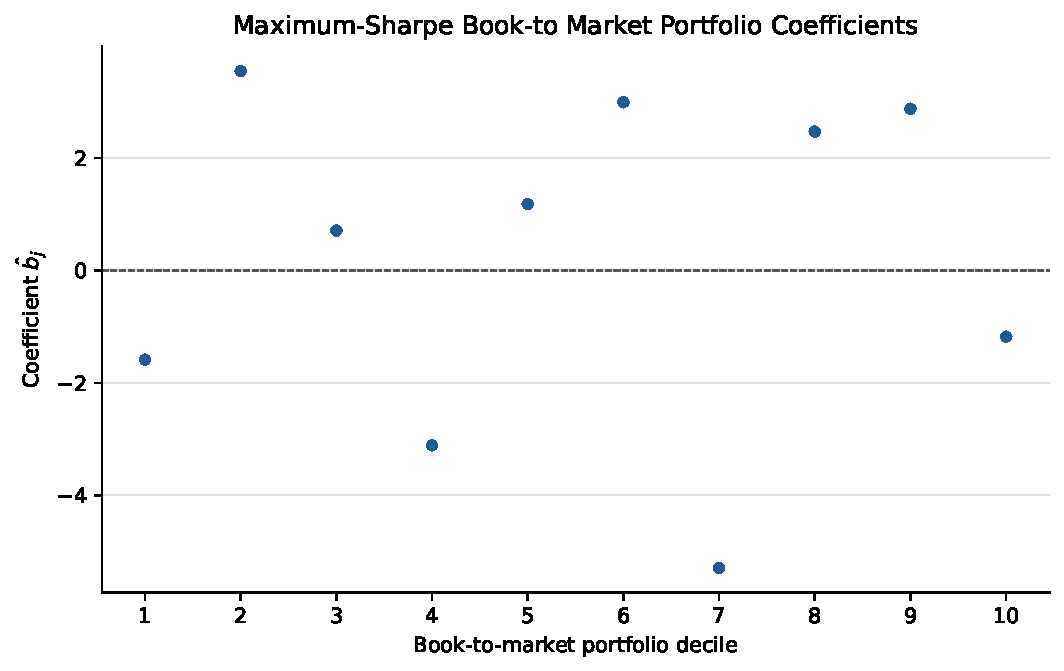
\includegraphics[width=0.75\textwidth]{results/q2a_b_coefficients.pdf}
    \caption{Estimated \(b\) coefficients across book-to-market decile portfolios}
    \label{fig:q2a_b}
\end{figure}

The estimated coefficients vary substantially across the book-to-market deciles and are not monotonic. This pattern arises because
\[
\hat b=\hat\Sigma^{-1}\hat\mu,
\]
so each coefficient depends not only on the average excess return of that portfolio, but also on its covariance with the other portfolios. Therefore, the coefficients do not simply increase or decrease with the book-to-market decile.






\subsection{Q2(b)}

The analysis in Q2(a) is repeated using the 10 value-weighted momentum decile portfolios.


The estimate of the constant is
\[
\hat a=1.0666,
\]
and the sample pricing condition
\[
\hat E[\hat M_t^*xR_t]\approx 0
\]
is satisfied.

Figure~\ref{fig:q2b_b} plots the estimated \(\hat b\) coefficients across the 10 momentum deciles.

\begin{figure}[H]
    \centering
    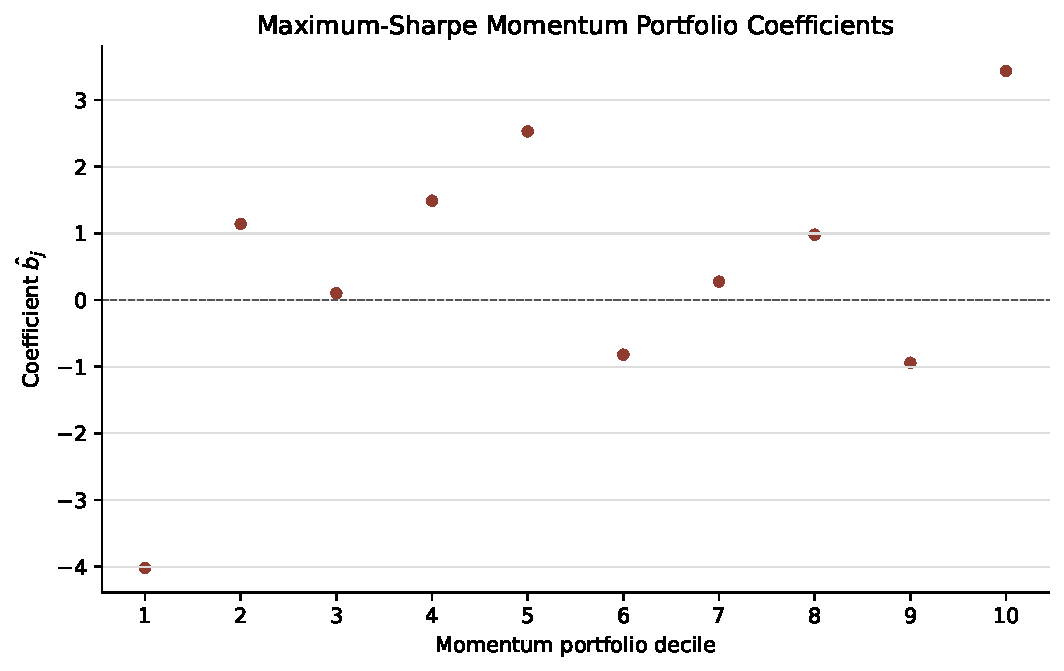
\includegraphics[width=0.75\textwidth]{results/q2b_b_coefficients.pdf}
    \caption{Estimated \(b\) coefficients across momentum decile portfolios}
    \label{fig:q2b_b}
\end{figure}

The estimated coefficients vary substantially across the momentum deciles and are not monotonic. As in Q2(a), this reflects both the average excess returns and the covariance structure across the portfolios.

The correlation between the SDF from Q2(a) and the SDF from Q2(b) is
\[
\operatorname{Corr}
\left(
M_{BM}^*,M_{MOM}^*
\right)
=
0.3555.
\]

The positive correlation indicates that the two SDFs share some common variation, but the relatively low correlation suggests that the book-to-market and momentum portfolios contain different information about the maximum Sharpe ratio direction.








\subsection{Q2(c)}

The 10 book-to-market portfolios and 10 momentum portfolios are combined to construct the SDF using 20 excess returns.


The estimate of the constant is

\[
\hat a=1.0927.
\]

The sample pricing condition
\[
\hat E[\hat M_t^*xR_t]\approx 0
\]
is satisfied for all 20 portfolios.

Figure~\ref{fig:q2c_b} plots the estimated \(\hat b\) coefficients for the book-to-market and momentum portfolios.

\begin{figure}[H]
    \centering
    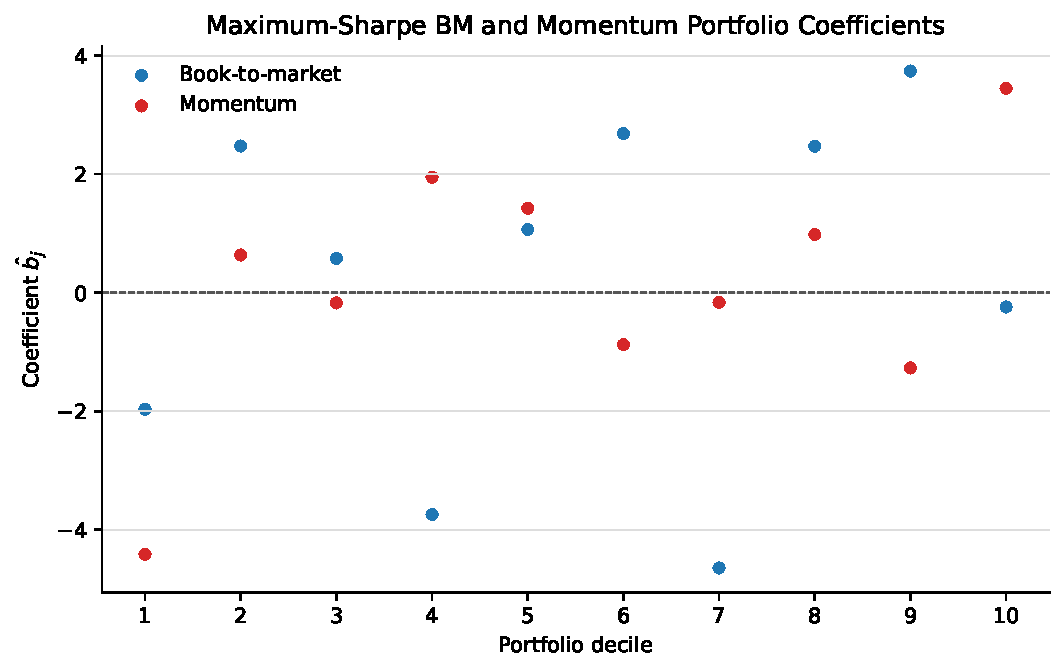
\includegraphics[width=0.75\textwidth]{results/q2c_b_coefficients.pdf}
    \caption{Estimated \(b\) coefficients for book-to-market and momentum portfolios}
    \label{fig:q2c_b}
\end{figure}

The coefficients vary substantially across both sets of portfolios and are not monotonic. This is because the coefficients depend on both the average excess returns and the covariance structure across all 20 portfolios.

The monthly Sharpe ratios of the maximum Sharpe ratio portfolios are
\[
SR_{BM}=0.1919,
\qquad
SR_{MOM}=0.2581,
\qquad
SR_{BM+MOM}=0.3045.
\]

The Sharpe ratio is highest when the book-to-market and momentum portfolios are combined. This is because the larger set of assets gives more opportunities to construct the maximum Sharpe ratio portfolio. The combined set includes both the BM and momentum portfolios, so its maximum Sharpe ratio cannot be lower than the maximum Sharpe ratio obtained from either set alone.




\subsection{Q2(d)}

For each of the 20 portfolios, the pricing error is calculated under the SDFs from Q2(a), Q2(b), and Q2(c) as
\[
\hat\alpha_p
=
\hat E[xR_p]
-
\widehat{\operatorname{Cov}}(-M^*,xR_p).
\]

\begin{table}[htbp]
\centering
\caption{Pricing errors under the Q2(a), Q2(b), and Q2(c) SDFs.}
\label{tab:q2d-pricing-errors}
\begin{tabular}{lrrr}
\hline
Portfolio & $\widehat{\alpha}^{Q2(a)}$ & $\widehat{\alpha}^{Q2(b)}$ & $\widehat{\alpha}^{Q2(c)}$ \\
\hline
BM: Lo 10 & 0.000000 & -0.001511 & 0.000000 \\
BM: 2-Dec & 0.000000 & -0.000101 & 0.000000 \\
BM: 3-Dec & 0.000000 & -0.000223 & 0.000000 \\
BM: 4-Dec & 0.000000 & -0.000778 & 0.000000 \\
BM: 5-Dec & 0.000000 & 0.000504 & 0.000000 \\
BM: 6-Dec & 0.000000 & 0.001261 & 0.000000 \\
BM: 7-Dec & 0.000000 & 0.000281 & 0.000000 \\
BM: 8-Dec & 0.000000 & 0.002376 & 0.000000 \\
BM: 9-Dec & 0.000000 & 0.003450 & 0.000000 \\
BM: Hi 10 & 0.000000 & 0.003198 & 0.000000 \\
MOM: Lo PRIOR & -0.010157 & 0.000000 & 0.000000 \\
MOM: PRIOR 2 & -0.005051 & 0.000000 & 0.000000 \\
MOM: PRIOR 3 & -0.003272 & 0.000000 & 0.000000 \\
MOM: PRIOR 4 & -0.001488 & 0.000000 & 0.000000 \\
MOM: PRIOR 5 & -0.000882 & 0.000000 & 0.000000 \\
MOM: PRIOR 6 & -0.000263 & 0.000000 & 0.000000 \\
MOM: PRIOR 7 & 0.000509 & 0.000000 & 0.000000 \\
MOM: PRIOR 8 & 0.001902 & 0.000000 & 0.000000 \\
MOM: PRIOR 9 & 0.002240 & 0.000000 & 0.000000 \\
MOM: Hi PRIOR & 0.005418 & 0.000000 & 0.000000 \\
\hline
\end{tabular}
\end{table}


The SDF from Q2(a) prices the 10 book-to-market portfolios almost exactly in sample, but produces larger pricing errors for the momentum portfolios. The SDF from Q2(b) prices the momentum portfolios almost exactly but produces pricing errors for the book-to-market portfolios.

The SDF from Q2(c) prices all 20 portfolios almost exactly, with pricing errors close to zero. This is because the Q2(c) SDF is constructed using both the book-to-market and momentum portfolios, while the SDFs in Q2(a) and Q2(b) are constructed using only one set of portfolios.

\subsection{Q2(e)}

The SDF coefficients are estimated using the sample from July 1927 to December 1989. These coefficients are then held fixed and used to construct the out-of-sample SDF from January 1990 onward. 

For each of the 20 portfolios, the out-of-sample pricing error is calculated as
\[
\hat\alpha_p^{OS}
=
\hat E_{OS}[xR_p]
-
\widehat{\operatorname{Cov}}_{OS}(-M^{*}_{OS},xR_p).
\]

\begin{table}[htbp]
\centering
\caption{Out-of-sample pricing errors for the Q2(e) SDF.}
\label{tab:q2e-pricing-errors}
\begin{tabular}{lr}
\hline
Portfolio & $\widehat{\alpha}_{OS}$ \\
\hline
BM: Lo 10 & 0.010971 \\
BM: 2-Dec & 0.007858 \\
BM: 3-Dec & 0.009002 \\
BM: 4-Dec & 0.006957 \\
BM: 5-Dec & 0.007986 \\
BM: 6-Dec & 0.007178 \\
BM: 7-Dec & 0.006977 \\
BM: 8-Dec & 0.005923 \\
BM: 9-Dec & 0.008269 \\
BM: Hi 10 & 0.009709 \\
MOM: Lo PRIOR & 0.027055 \\
MOM: PRIOR 2 & 0.016483 \\
MOM: PRIOR 3 & 0.013905 \\
MOM: PRIOR 4 & 0.012077 \\
MOM: PRIOR 5 & 0.009180 \\
MOM: PRIOR 6 & 0.008297 \\
MOM: PRIOR 7 & 0.007601 \\
MOM: PRIOR 8 & 0.006444 \\
MOM: PRIOR 9 & 0.004322 \\
MOM: Hi PRIOR & 0.005453 \\
\hline
\end{tabular}
\end{table}


The out-of-sample pricing errors are much larger than the in-sample pricing errors in Q2(d). The average absolute pricing error is about \(0.81\%\) per month for the book-to-market portfolios and \(1.11\%\) per month for the momentum portfolios.

Overall, the SDF estimated using pre-1990 data does not price the 20 portfolios as well after 1990. This suggests that the relation between the portfolio returns and the estimated SDF is not stable across the two sample periods.

\newpage


\section{Q3}


\subsection{Q3(a)}

The investor solves

\[
\max_{\omega_t}
E_t[U(W_{t+1})]
\]

subject to

\[
W_{t+1}
=
W_t\omega_t'R_{t+1}
\]

and

\[
\mathbf{1}'\omega_t=1.
\]

The Lagrangian is

\[
\mathcal{L}
=
E_t
\left[
U\left(
W_t\omega_t'R_{t+1}
\right)
\right]
+
\lambda_t
\left(
1-\mathbf{1}'\omega_t
\right).
\]

Taking the derivative with respect to \(\omega_t\), the first-order condition is

\[
\frac{\partial \mathcal{L}}{\partial \omega_t}
=
E_t
\left[
U'(W_{t+1})
W_tR_{t+1}
\right]
-
\lambda_t\mathbf{1}
=
0.
\]

Therefore, for any two assets \(j\) and \(k\),

\[
E_t
\left[
U'(W_{t+1})W_tR_{j,t+1}
\right]
=
E_t
\left[
U'(W_{t+1})W_tR_{k,t+1}
\right].
\]

Subtracting the right-hand side from the left-hand side gives

\[
E_t
\left[
U'(W_{t+1})W_t
\left(
R_{j,t+1}-R_{k,t+1}
\right)
\right]
=
0.
\]

Let asset \(k\) be the baseline asset \(R_{f,t+1}\). Then

\[
R_{j,t+1}-R_{f,t+1}
=
xR_{j,t+1}.
\]

Therefore,

\[
E_t
\left[
U'(W_{t+1})W_t
xR_{j,t+1}
\right]
=
0.
\]

Under CRRA utility,

\[
U(W)
=
\frac{W^{1-\gamma}}{1-\gamma}.
\]

Therefore, marginal utility is

\[
U'(W)
=
W^{-\gamma}.
\]

Hence,

\[
U'(W_{t+1})
=
W_{t+1}^{-\gamma}.
\]

Since

\[
W_{t+1}
=
W_tR_{w,t+1},
\]

we have

\[
U'(W_{t+1})
=
\left(
W_tR_{w,t+1}
\right)^{-\gamma}.
\]

Thus,

\[
U'(W_{t+1})
=
W_t^{-\gamma}
R_{w,t+1}^{-\gamma}.
\]

Substituting this into the first-order condition gives

\[
E_t
\left[
W_t^{-\gamma}
R_{w,t+1}^{-\gamma}
W_t
xR_{j,t+1}
\right]
=
0.
\]

Combining the powers of \(W_t\),

\[
E_t
\left[
W_t^{1-\gamma}
R_{w,t+1}^{-\gamma}
xR_{j,t+1}
\right]
=
0.
\]

Since \(W_t\) is known at time \(t\), \(W_t^{1-\gamma}\) can be taken outside the conditional expectation:

\[
W_t^{1-\gamma}
E_t
\left[
R_{w,t+1}^{-\gamma}
xR_{j,t+1}
\right]
=
0.
\]

Since

\[
W_t^{1-\gamma}\neq 0,
\]

it follows that

\[
E_t
\left[
R_{w,t+1}^{-\gamma}
xR_{j,t+1}
\right]
=
0.
\]

This holds for every asset \(j\). Therefore, in vector form,

\[
\boxed{
E_t
\left[
R_{w,t+1}^{-\gamma}
xR_{t+1}
\right]
=
0.
}
\]

Thus, the SDF

\[
\boxed{
M_{t+1}
=
R_{w,t+1}^{-\gamma}
}
\]

prices the vector of excess returns.




\subsection{Q3(b)}

Using the unconditional SDF moment condition

\[
E\left[R_{w,t}^{-\gamma}xR_{w,t}\right]=0,
\]

with

\[
R_{w,t}=e^{re_t},
\qquad
R_{f,t}=e^{rf_t},
\qquad
xR_{w,t}=R_{w,t}-R_{f,t},
\]

\(\gamma\) is estimated by GMM using \(T=1129\) monthly observations.

The estimate is

\[
\hat{\gamma}=1.9061.
\]

The standard error is calculated using a Newey-West (1987, 1994) HAC estimator with a Bartlett kernel and a data-driven bandwidth. The selected bandwidth is

\[
L=23,
\]

which gives

\[
SE(\hat{\gamma})=0.5941.
\]

\subsection{Q3(c)}

Using the two unconditional SDF moment conditions

\[
E\left[R_{w,t}^{-\gamma}xR_{w,t}\right]=0
\]

and

\[
E\left[R_{w,t}^{-\gamma}
\left(z_{t-1}xR_{w,t}\right)\right]=0,
\]

\(\gamma\) is estimated by GMM with an identity weighting matrix using \(T=973\) monthly observations.

The estimate is

\[
\hat{\gamma}=2.9851,
\]

with a Newey-West standard error of

\[
SE(\hat{\gamma})=0.7150.
\]

The two pricing errors and their t-statistics are

\[
\begin{array}{lcc}
\hline
& \text{Pricing Error} & t\text{-statistic}\\
\hline
\text{Wealth portfolio} & -0.00312 & -0.802\\
\text{Managed portfolio} & 0.00223 & 0.802\\
\hline
\end{array}
\]

The data-driven Newey-West procedure selects

\[
L=22.
\]

The joint test that the two pricing errors are zero gives

\[
\chi^2(1)=0.644,
\qquad
p=0.422.
\]

Thus, the null hypothesis that the pricing errors are jointly zero cannot be rejected. This suggests that the CRRA SDF is broadly consistent with both the wealth-portfolio and managed-portfolio moment conditions.

\subsection{Q3(d)}

Using the same two moment conditions as in Q3(c), \(\gamma\) is re-estimated using two-step GMM. In the second step, the inverse of the Newey-West long-run covariance matrix from the first step is used as the weighting matrix.

Using \(T=973\) observations, the two-step GMM estimate is

\[
\hat{\gamma}=2.9448,
\]

with a Newey-West standard error of

\[
SE(\hat{\gamma})=0.7169.
\]

The pricing errors for the wealth portfolio and the managed portfolio are

\[
-0.00182
\quad\text{and}\quad
0.00404,
\]

with corresponding t-statistics of

\[
-0.802
\quad\text{and}\quad
0.802.
\]

The first-step Newey-West procedure selects

\[
L=22.
\]

The joint test that the two pricing errors are zero gives

\[
\chi^2(1)=0.6440,
\qquad
p=0.4223.
\]

Thus, the null hypothesis that the pricing errors are jointly zero cannot be rejected. This suggests that the two-step GMM specification remains consistent with the two pricing conditions considered here.


\subsection{Q3(e)}

Using the wealth portfolio together with the 10 book-to-market and 10 momentum decile portfolios, \(\gamma\) is estimated by GMM using 21 unconditional moment conditions.

Using \(T=1129\) monthly observations, the GMM estimate is

\[
\hat{\gamma}=1.9083,
\]

with a Newey-West standard error of

\[
SE(\hat{\gamma})=0.5863.
\]

The data-driven Newey-West procedure selects

\[
L=23.
\]

The pricing errors and corresponding t-statistics for the wealth portfolio, the 10 book-to-market portfolios, and the 10 momentum portfolios are reported below.

\begin{table}[htbp]
\centering
\small
\caption{Pricing errors for the Q3(e) identity-weighted GMM model.}
\label{tab:q3e-pricing-errors}
\begin{tabular}{lrrr}
\hline
Portfolio & Pricing error & Standard error & $t$-statistic \\
\hline
Wealth portfolio ($xR_w$) & -0.000108 & 0.002904 & -0.037 \\
BM Lo 10 & -0.001137 & 0.001284 & -0.885 \\
BM 2-Dec & 0.000604 & 0.001060 & 0.570 \\
BM 3-Dec & 0.000542 & 0.001443 & 0.375 \\
BM 4-Dec & -0.000669 & 0.001380 & -0.485 \\
BM 5-Dec & 0.000588 & 0.001557 & 0.378 \\
BM 6-Dec & 0.000769 & 0.001665 & 0.462 \\
BM 7-Dec & -0.000233 & 0.002005 & -0.116 \\
BM 8-Dec & 0.001699 & 0.002066 & 0.822 \\
BM 9-Dec & 0.003217 & 0.002796 & 1.151 \\
BM Hi 10 & 0.001712 & 0.003112 & 0.550 \\
MOM Lo PRIOR & -0.006566 & 0.003240 & -2.026 \\
MOM PRIOR 2 & -0.002502 & 0.002488 & -1.006 \\
MOM PRIOR 3 & -0.001939 & 0.002186 & -0.887 \\
MOM PRIOR 4 & -0.001148 & 0.001864 & -0.616 \\
MOM PRIOR 5 & -0.000097 & 0.001533 & -0.063 \\
MOM PRIOR 6 & 0.000111 & 0.001519 & 0.073 \\
MOM PRIOR 7 & 0.000546 & 0.001283 & 0.426 \\
MOM PRIOR 8 & 0.001469 & 0.001030 & 1.426 \\
MOM PRIOR 9 & 0.001904 & 0.001266 & 1.503 \\
MOM Hi PRIOR & 0.004200 & 0.001377 & 3.051 \\
\hline
\end{tabular}
\end{table}


The joint test that all 21 pricing errors are zero gives

\[
\chi^2(20)=92.1354,
\qquad
p<0.0001.
\]

Thus, the null hypothesis that all pricing errors are jointly zero is rejected. This suggests that the CRRA SDF is not able to jointly price the wealth, book-to-market, and momentum portfolios, with the strongest evidence of mispricing coming from the momentum portfolios.


\newpage

\section{Q4}



\subsection{Q4(a)}

From Q3(a), the nonlinear SDF is

\[
M_{t+1}
=
R_{w,t+1}^{-\gamma}.
\]

Let

\[
\mu_t
=
E_t[R_{w,t+1}].
\]

Define

\[
f(R)
=
R^{-\gamma}.
\]

Then

\[
f'(R)
=
-\gamma R^{-\gamma-1}.
\]

Using a first-order Taylor expansion of \(R_{w,t+1}^{-\gamma}\) around \(\mu_t\),

\[
f(R_{w,t+1})
\approx
f(\mu_t)
+
f'(\mu_t)
\left(
R_{w,t+1}-\mu_t
\right).
\]

Therefore,

\[
M_{t+1}
=
R_{w,t+1}^{-\gamma}
\]

can be approximated by

\[
M_{t+1}
\approx
\mu_t^{-\gamma}
-
\gamma
\mu_t^{-\gamma-1}
\left(
R_{w,t+1}-\mu_t
\right).
\]

Expanding the last term,

\[
M_{t+1}
\approx
\mu_t^{-\gamma}
-
\gamma
\mu_t^{-\gamma-1}
R_{w,t+1}
+
\gamma
\mu_t^{-\gamma-1}\mu_t.
\]

Since

\[
\mu_t^{-\gamma-1}\mu_t
=
\mu_t^{-\gamma},
\]

we obtain

\[
M_{t+1}
\approx
\mu_t^{-\gamma}
+
\gamma\mu_t^{-\gamma}
-
\gamma\mu_t^{-\gamma-1}R_{w,t+1}.
\]

Therefore,

\[
M_{t+1}
\approx
(1+\gamma)\mu_t^{-\gamma}
-
\gamma\mu_t^{-\gamma-1}R_{w,t+1}.
\]

Comparing this expression with

\[
M_{t+1}
\approx
a_t-b_tR_{w,t+1},
\]

we have

\[
\boxed{
a_t
=
(1+\gamma)\mu_t^{-\gamma}
}
\]

and

\[
\boxed{
b_t
=
\gamma\mu_t^{-\gamma-1}.
}
\]

Since

\[
\mu_t
=
E_t[R_{w,t+1}],
\]

these can equivalently be written as

\[
\boxed{
a_t
=
(1+\gamma)
\left(
E_t[R_{w,t+1}]
\right)^{-\gamma}
}
\]

and

\[
\boxed{
b_t
=
\gamma
\left(
E_t[R_{w,t+1}]
\right)^{-\gamma-1}.
}
\]

Therefore,

\[
\boxed{
M_{t+1}
\approx
a_t-b_tR_{w,t+1}.
}
\]

The advantage of this linear SDF is that it is linear in \(R_{w,t+1}\), which leads to a simpler GMM estimator.

One disadvantage is that the linear SDF can become negative when \(R_{w,t+1}\) is sufficiently large:

\[
a_t-b_tR_{w,t+1}<0.
\]

In contrast, the original power-utility SDF

\[
M_{t+1}
=
R_{w,t+1}^{-\gamma}
\]

is always positive as long as

\[
R_{w,t+1}>0.
\]


\subsection{Q4(b)}

Using the normalized linear SDF

\[
M_t
=
1-b\left(R_{w,t}-E[R_w]\right),
\]

\(b\) is estimated by GMM using the wealth portfolio together with the 10 book-to-market and 10 momentum decile portfolios, for a total of 21 unconditional moment conditions. An identity weighting matrix is used.

Using \(T=1129\) monthly observations from December 1927 to December 2021, the GMM estimate is

\[
\hat b=2.0141,
\]

with a Newey-West standard error of

\[
SE(\hat b)=0.6001.
\]

The data-driven Newey-West procedure selects

\[
L=23.
\]

The pricing errors and corresponding t-statistics for the wealth portfolio, the 10 book-to-market portfolios, and the 10 momentum portfolios are reported below.

\begin{table}[htbp]
\centering
\small
\caption{Identity-weighted GMM results for the normalized linear SDF.}
\label{tab:q4b-results}
\begin{tabular}{lrr}
\hline
Quantity or portfolio & Estimate & $t$-statistic \\
\hline
$\widehat{b}$ & 2.014081 & \\
Newey-West standard error of $\widehat{b}$ & 0.600057 & \\
Observations & 1129 & \\
Common bandwidth $L$ & 23 & \\
Joint $\chi^2(20)$ & 103.976951 & \\
Joint-test $p$-value & 2.430e-13 & \\
\hline
\multicolumn{3}{l}{\textit{Pricing errors}} \\
\hline
Wealth portfolio ($xR_w$) & -0.000808 & -0.359 \\
BM Lo 10 & -0.000379 & -0.285 \\
BM 2-Dec & 0.001451 & 1.303 \\
BM 3-Dec & 0.000991 & 0.767 \\
BM 4-Dec & -0.000164 & -0.127 \\
BM 5-Dec & 0.000801 & 0.577 \\
BM 6-Dec & 0.001224 & 0.843 \\
BM 7-Dec & -0.000437 & -0.257 \\
BM 8-Dec & 0.001494 & 0.892 \\
BM 9-Dec & 0.002587 & 1.183 \\
BM Hi 10 & 0.001103 & 0.411 \\
MOM Lo PRIOR & -0.007001 & -2.394 \\
MOM PRIOR 2 & -0.001644 & -0.736 \\
MOM PRIOR 3 & -0.000851 & -0.411 \\
MOM PRIOR 4 & -0.000153 & -0.088 \\
MOM PRIOR 5 & 0.000850 & 0.614 \\
MOM PRIOR 6 & 0.000788 & 0.581 \\
MOM PRIOR 7 & 0.000948 & 0.751 \\
MOM PRIOR 8 & 0.001821 & 1.866 \\
MOM PRIOR 9 & 0.002194 & 1.833 \\
MOM Hi PRIOR & 0.004591 & 3.271 \\
\hline
\end{tabular}
\end{table}


The joint test that all 21 pricing errors are zero gives

\[
\chi^2(20)=103.9770,
\qquad
p=2.43\times10^{-13}.
\]

Thus, the null hypothesis that all pricing errors are jointly zero is strongly rejected. This suggests that the linear SDF is not able to jointly price the wealth, book-to-market, and momentum portfolios.


\subsection{Q4(c)}

Using the same 21 moment conditions as in Q4(b), \(b\) is re-estimated using efficient GMM. The inverse of the Newey-West long-run covariance matrix from Q4(b) is used as the weighting matrix.

The sample moment condition can be written as

\[
\bar g(b)
=
\hat\mu-b\hat c,
\]

where

\[
\hat\mu
=
\hat E[xR_t]
\]

and

\[
\hat c
=
\hat E\left[
(R_{w,t}-\bar R_w)xR_t
\right].
\]

Using the efficient weighting matrix

\[
W=\hat S^{-1},
\]

the GMM objective function is

\[
Q(b)
=
(\hat\mu-b\hat c)'
\hat S^{-1}
(\hat\mu-b\hat c).
\]

Taking the derivative with respect to \(b\),

\[
\frac{\partial Q(b)}{\partial b}
=
-2\hat c'
\hat S^{-1}
(\hat\mu-b\hat c).
\]

Setting the first-order condition equal to zero gives

\[
\hat c'
\hat S^{-1}
(\hat\mu-\hat b_{\mathrm{eff}}\hat c)
=
0.
\]

Therefore, the efficient GMM estimator has the analytical expression

\[
\hat b_{\mathrm{eff}}
=
\frac{
\hat c'\hat S^{-1}\hat\mu
}{
\hat c'\hat S^{-1}\hat c
}.
\]

Using \(T=1129\) monthly observations, the efficient GMM estimate is

\[
\hat b_{\mathrm{eff}}=2.5984,
\]

with a Newey-West standard error of

\[
SE(\hat b_{\mathrm{eff}})=0.4582.
\]

The pricing errors and corresponding t-statistics for the wealth portfolio, the 10 book-to-market portfolios, and the 10 momentum portfolios are reported below.

\begin{table}[htbp]
\centering
\small
\caption{Efficient GMM results for the normalized linear SDF.}
\label{tab:q4c-results}
\begin{tabular}{lrr}
\hline
Quantity or portfolio & Estimate & $t$-statistic \\
\hline
$\widehat{b}_{eff}$ & 2.598366 & \\
Newey-West standard error of $\widehat{b}_{eff}$ & 0.458231 & \\
Observations & 1129 & \\
Q4(b) common bandwidth $L$ & 23 & \\
Joint $\chi^2(20)$ & 103.976951 & \\
Joint-test $p$-value & 2.430e-13 & \\
\hline
\multicolumn{3}{l}{\textit{Pricing errors}} \\
\hline
Wealth portfolio ($xR_w$) & -0.025407 & -1.548 \\
BM Lo 10 & -0.002267 & -1.133 \\
BM 2-Dec & -0.000264 & -0.157 \\
BM 3-Dec & -0.000675 & -0.427 \\
BM 4-Dec & -0.002179 & -1.053 \\
BM 5-Dec & -0.001080 & -0.521 \\
BM 6-Dec & -0.000764 & -0.342 \\
BM 7-Dec & -0.002561 & -1.077 \\
BM 8-Dec & -0.000761 & -0.359 \\
BM 9-Dec & 0.000294 & 0.135 \\
BM Hi 10 & -0.001595 & -0.609 \\
MOM Lo PRIOR & -0.009314 & -2.740 \\
MOM PRIOR 2 & -0.003518 & -1.342 \\
MOM PRIOR 3 & -0.002566 & -0.962 \\
MOM PRIOR 4 & -0.002019 & -0.855 \\
MOM PRIOR 5 & -0.000831 & -0.459 \\
MOM PRIOR 6 & -0.000981 & -0.510 \\
MOM PRIOR 7 & -0.000963 & -0.494 \\
MOM PRIOR 8 & -0.000124 & -0.077 \\
MOM PRIOR 9 & 0.000170 & 0.098 \\
MOM Hi PRIOR & 0.002436 & 1.320 \\
\hline
\end{tabular}
\end{table}


The joint test that all 21 pricing errors are zero gives

\[
\chi^2(20)=103.9770,
\qquad
p=2.43\times10^{-13}.
\]

Thus, the null hypothesis that all pricing errors are jointly zero is strongly rejected. This suggests that the efficiently estimated linear SDF is not able to jointly price the wealth, book-to-market, and momentum portfolios.

\subsection{Q4(d)}

The linear SDF

\[
M_t=a-bR_{w,t}
\]

implies a linear beta-pricing model. For each of the 21 assets, the time-series regression

\[
xR_{j,t}
=
\alpha_j+\beta_j R_{w,t}+\epsilon_{j,t}
\]

is estimated, where \(\alpha_j\) measures the pricing error.

The factor risk premium is estimated from a time-series regression of \(R_{w,t}\) on a constant. Using \(T=1129\) monthly observations, the estimate is

\[
\hat{\lambda}=1.0877,
\]

with a Newey-West standard error of

\[
SE(\hat{\lambda})=0.0180.
\]

The data-driven Newey-West procedure selects

\[
L=23.
\]

The estimated pricing errors and corresponding Newey-West t-statistics for the wealth portfolio, the 10 book-to-market portfolios, and the 10 momentum portfolios are reported below.

\begin{table}[htbp]
\centering
\small
\caption{Time-series beta-pricing results for the linear SDF model.}
\label{tab:q4d-results}
\begin{tabular}{lrr}
\hline
Quantity or portfolio & Estimate & $t$-statistic \\
\hline
$\widehat{\lambda}$ & 1.087734 & \\
Newey-West standard error of $\widehat{\lambda}$ & 0.017994 & \\
Lambda bandwidth $L$ & 23 & \\
Observations & 1129 & \\
GRS $F(21,1107)$ & 1319.663199 & \\
GRS $p$-value & $2.391\times 10^{-764}$ & \\
\hline
\multicolumn{3}{l}{\textit{Time-series regression alphas}} \\
\hline
Wealth portfolio ($xR_w$) & -0.999425 & -30.945 \\
BM Lo 10 & -0.077025 & -7.751 \\
BM 2-Dec & -0.068177 & -7.956 \\
BM 3-Dec & -0.066631 & -7.254 \\
BM 4-Dec & -0.081969 & -6.568 \\
BM 5-Dec & -0.075541 & -6.313 \\
BM 6-Dec & -0.079485 & -6.256 \\
BM 7-Dec & -0.086628 & -6.217 \\
BM 8-Dec & -0.090069 & -6.152 \\
BM 9-Dec & -0.090472 & -5.705 \\
BM Hi 10 & -0.108431 & -5.450 \\
MOM Lo PRIOR & -0.100904 & -4.308 \\
MOM PRIOR 2 & -0.077742 & -4.789 \\
MOM PRIOR 3 & -0.070453 & -4.949 \\
MOM PRIOR 4 & -0.075904 & -5.695 \\
MOM PRIOR 5 & -0.067373 & -6.425 \\
MOM PRIOR 6 & -0.071037 & -6.241 \\
MOM PRIOR 7 & -0.076635 & -7.300 \\
MOM PRIOR 8 & -0.077156 & -8.411 \\
MOM PRIOR 9 & -0.079958 & -8.302 \\
MOM Hi PRIOR & -0.082897 & -8.969 \\
\hline
\end{tabular}
\end{table}


The GRS test of the null hypothesis

\[
H_0:
\alpha_1=\alpha_2=\cdots=\alpha_{21}=0
\]

gives

\[
GRS=1319.6632,
\qquad
p<0.0001.
\]

Thus, the null hypothesis that all pricing errors are jointly zero is strongly rejected. This suggests that the linear beta-pricing model does not jointly price the wealth, book-to-market, and momentum portfolios.


\subsection{Q4(e)}

The linear beta-pricing model is estimated using Fama--MacBeth regressions. First, the factor loadings \(\beta_j\) are estimated for the 21 assets. Then, a cross-sectional regression is run in each month to obtain the factor risk premium \(\lambda_t\) and the corresponding pricing errors \(\alpha_{j,t}\).

The Fama--MacBeth estimate of the factor risk premium is

\[
\hat{\lambda}
=
\frac{1}{T}\sum_{t=1}^{T}\hat{\lambda}_t
=
0.0851.
\]

The standard error is calculated from a time-series regression of \(\hat{\lambda}_t\) on a constant using Newey-West standard errors. The resulting standard error is

\[
SE(\hat{\lambda})=0.0186.
\]

The data-driven Newey-West procedure selects

\[
L=23,
\]

using \(T=1129\) monthly observations.

For each asset \(j\), the average pricing error is

\[
\hat{\alpha}_j
=
\frac{1}{T}
\sum_{t=1}^{T}
\hat{\alpha}_{j,t},
\]

and its t-statistic is calculated using Newey-West standard errors from a time-series regression of \(\hat{\alpha}_{j,t}\) on a constant.

The factor risk premium estimate and the pricing errors and corresponding t-statistics for the wealth portfolio, the 10 book-to-market portfolios, and the 10 momentum portfolios are reported below.

\begin{table}[htbp]
\centering
\small
\caption{Fama--MacBeth results for the linear beta-pricing model.}
\label{tab:q4e-results}
\begin{tabular}{lrr}
\hline
Quantity or portfolio & Estimate & $t$-statistic \\
\hline
$\widehat{\lambda}$ & 0.085133 & \\
Newey-West standard error of $\widehat{\lambda}$ & 0.018579 & \\
Lambda bandwidth $L$ & 23 & \\
Observations & 1129 & \\
\hline
\multicolumn{3}{l}{\textit{Average cross-sectional pricing errors}} \\
\hline
Wealth portfolio ($xR_w$) & -0.000808 & -0.444 \\
BM Lo 10 & -0.000379 & -0.313 \\
BM 2-Dec & 0.001451 & 1.484 \\
BM 3-Dec & 0.000991 & 0.871 \\
BM 4-Dec & -0.000164 & -0.143 \\
BM 5-Dec & 0.000801 & 0.659 \\
BM 6-Dec & 0.001224 & 1.192 \\
BM 7-Dec & -0.000437 & -0.342 \\
BM 8-Dec & 0.001494 & 1.115 \\
BM 9-Dec & 0.002587 & 1.502 \\
BM Hi 10 & 0.001103 & 0.490 \\
MOM Lo PRIOR & -0.007001 & -2.781 \\
MOM PRIOR 2 & -0.001644 & -0.832 \\
MOM PRIOR 3 & -0.000851 & -0.550 \\
MOM PRIOR 4 & -0.000153 & -0.106 \\
MOM PRIOR 5 & 0.000850 & 0.749 \\
MOM PRIOR 6 & 0.000788 & 0.649 \\
MOM PRIOR 7 & 0.000948 & 0.925 \\
MOM PRIOR 8 & 0.001821 & 1.905 \\
MOM PRIOR 9 & 0.002194 & 1.822 \\
MOM Hi PRIOR & 0.004591 & 3.151 \\
\hline
\end{tabular}
\end{table}


Most pricing errors are not statistically significant. However, the lowest momentum portfolio has a significantly negative pricing error, while the highest momentum portfolio has a significantly positive pricing error. This suggests that the linear beta-pricing model does not fully capture the return spread across the momentum portfolios.


\end{document}
